\documentclass[12pt, letterpaper, oneside]{article}
\usepackage[utf8]{inputenc}
\usepackage{setspace}
\usepackage{graphicx}
\usepackage{float}
\usepackage[parfill]{parskip}
\floatstyle{boxed}
\restylefloat{figure}
\onehalfspacing
\setlength{\parindent}{0pt}
%\linespread{1.3}
 
\title{\textbf{Human Factors in Unmanned Aerial Systems (UAS)}}
\author{Dritan Hasani\\
		Department of Computer Science and Engineering,\\
		University of Nevada, Reno\\
		\texttt{dhasani@nevada.unr.edu}\\
		{+1 775 223 6257}}
\date{}
 
\begin{document}
 
\begin{titlepage}
\maketitle
\thispagestyle{empty}
\end{titlepage}
 
\section{HISTORY}
Even though it might seem like the unmanned aerial vehicles (UAVs) are only a recent technology, the truth is that research in the field of unmanned aerial systems has started as early as the beginning of the 20th century. Back in 1918 Charles Kettering has built the first prototype UAV for the needs of the US Army \cite{10}. At about the same time United Kingdom had built several UAVs for military use, and finally June 1921 brought the first successful demonstration of the radio-controlled assault drone \cite{16}. The interest for developing unmanned aerial systems remained with the military in the following decades and as a result several drones have been designed and deployed in military missions. The United States gave UAVs an increasing role in surveillance and reconnaissance missions during the Vietnam War in the 60's and 70's; Israel successfully used drones during the war against Syria in 80's, and so on. The successful depoloyment of drones in these military missions encouraged many other countries and governments to start investing in drone development programs, hence nowadays unmanned aerial vehicles hold an important and permanent position in the military arsenal of the US and many other countries across Europe, Middle East, and Asia.
  
In addition to the military usage there is also a great potential for using UAVs in numerous civilian applications. In the recent years the research and business communities became highly interested in exploring the possibilities of using UAVs for civilian applications such as fire fighting, search and rescue, surveillance, construction and building inspection, mapping, agriculture, and so on, and as a result a new class of low-cost, small-sized (multi-rotor) UAVs has emerged.

Despite the endless possibilitis for UAV usage there are numerous challenges that need to be addressed before their full potential can be utilized in the daily civilian applications. A number of technical challenges related to navigation, sensing, communication delays, bandwidth, autonomy, etc, need to be addressed before we see a wide expansion of UAV usage. In addition there is also safety concerns that are hindering the further development of unmanned systems. Williams (2004) suggests that the rate of accidents for UAVs is several times higher than for manned aircrafts \cite{19}. Because of these concerns US FAA has in place a set of regulations that make it illegal to fly UAVs into the regular airspace or to conduct flights over densely populated areas. This fact imposes serious difficulties for the further research and development in the field of civilian UAV applications, therefore it is highly important for the regulators to move forward quickly in developing the necessary rules and regulations under which the UAVs will be finally allowed into the civilian airspace. Nevertheless, these technical and regulatory issues are beyond the scope of our work, therefore in the following sections we will focus solely on the issues related to the human factors that need to be considered in the design and deployment of unmanned aerial systems in disaster mitigation operations. 

\section{HUMAN FACTORS}
UAVs are promising for disaster mitigation tasks, yet there are numerous challenges that need to be addressed before their full potential can be utilized to assist first responders in their duties. Unmanned Vehicles (UV) are generally designed to operate in remote areas that are unreachable or potentially dangerous to the human personnel. In these scenarios it would be desirable to have unmanned vehicles capable of navigating, making decisions, exploring the area, and finally extracting and sending back important information autonomously. However though, the current technology is far from having achieved the level of competency that would allow UAVs to complete disaster mitigation missions in completely autonomous mode. Human involvement is necessary especially when it comes to decision making, perception of previously unknown situations, detection of anomalies, etc, but this involvement introduces new challenges that are related to the coordination of such mixed human-robot teams.

Early systems used \emph{teleoperation} as the main method for controlling the UAVs. In this approach the human operator sits at a ground station and maintains a full UAV control from the distance. The major drawback of \emph{teleoperation} is that it requires at least one human operator per UAV, possibly more depending on mission objectives. For example, some military UAVs require up to four human teleoperators plus the fifth one who specializes in takeoffs and landings \cite{33}. To eliminate this drawback the researchers have introduced the \emph{semi-autonomous control}, where the UAV and the human operator share the control over the system. In the general setup the UAV has a number of operations that it can perform, whereas the operator interacts with the system only to issue commands that will then be executed autonomously by the UAV. Previous research has shown that semi-autonomous aproach is best accepted by the emergency response community, therefore in this document we will be referring to the semi-autonomous aproach each time we talk about UAV control.    

In both cases, \emph{teleoperation} and \emph{semi-autonomous control}, the operator controls the UAV from a distance, therefore it is necessary to have some type of interface not only to issue commands but also to see what the UAV is doing. Previous work has addressed the issue of achieving multi-robot control through well-designed interfaces that take into account the cognitive and perceptual strengths and limitations of the human operators \cite{11, 25}. Others have focused on studying the user requirements and their implications for the interface design, showing that interfaces are often overloaded with unnecessary information causing most of the provided data to be neglected by the users \cite{7, 22}. The UAV literature generally discusses the human factors in terms of \emph{situational awareness} (SA) and \emph{operator cognitive load}, therefore when discussing the human factors associated with the design of interfaces for multiple UAV control our main focus will be on the human - UAV interaction in terms of cognitive load and situational awareness (SA). We will try to answer the question if the human factors have been adequately addressed in the current UAV development, and subsequently identify the best methods to design UAV interfaces and establish the appropriate levels of autonomy in order to optimize these two factors, i.e. maximize the performance while simultaneously reducing the workload of the human operator.   

\section{INTERFACE DESIGN}
A lot of research has been conducted to investigate different interface designs that provide for an easy navigation of UAVs in disaster mitigation scenarios. The proposed interfaces range from the ones that support graphical interaction, to those that utilize voice-based commands, motion tracking, and even ones that resemble the traditional aircraft cockpits \cite{8, 23, 24, 25}. There is no single type of interface that is best suited for all situations, but it is our belief that for a disaster mitigation mission a point-and-click graphical user interface (GUI) is the form of interaction that humans are mostly used to. One such interface, the open source \emph{QGroundControl} Ground Control Station (GCS)\footnote{www.qgroundcontrol.org} is presented in the Figure 1 below. An interface that is based on this type of interaction facilitates an intuitive and easy operation of the UAV, which is the precondition for a better situational awareness and lowered cognitive load of the human operator \cite{32}. 

\begin{figure}[h!]
  \caption{QGroundControl Ground Control Station (GCS).}
  \centering
    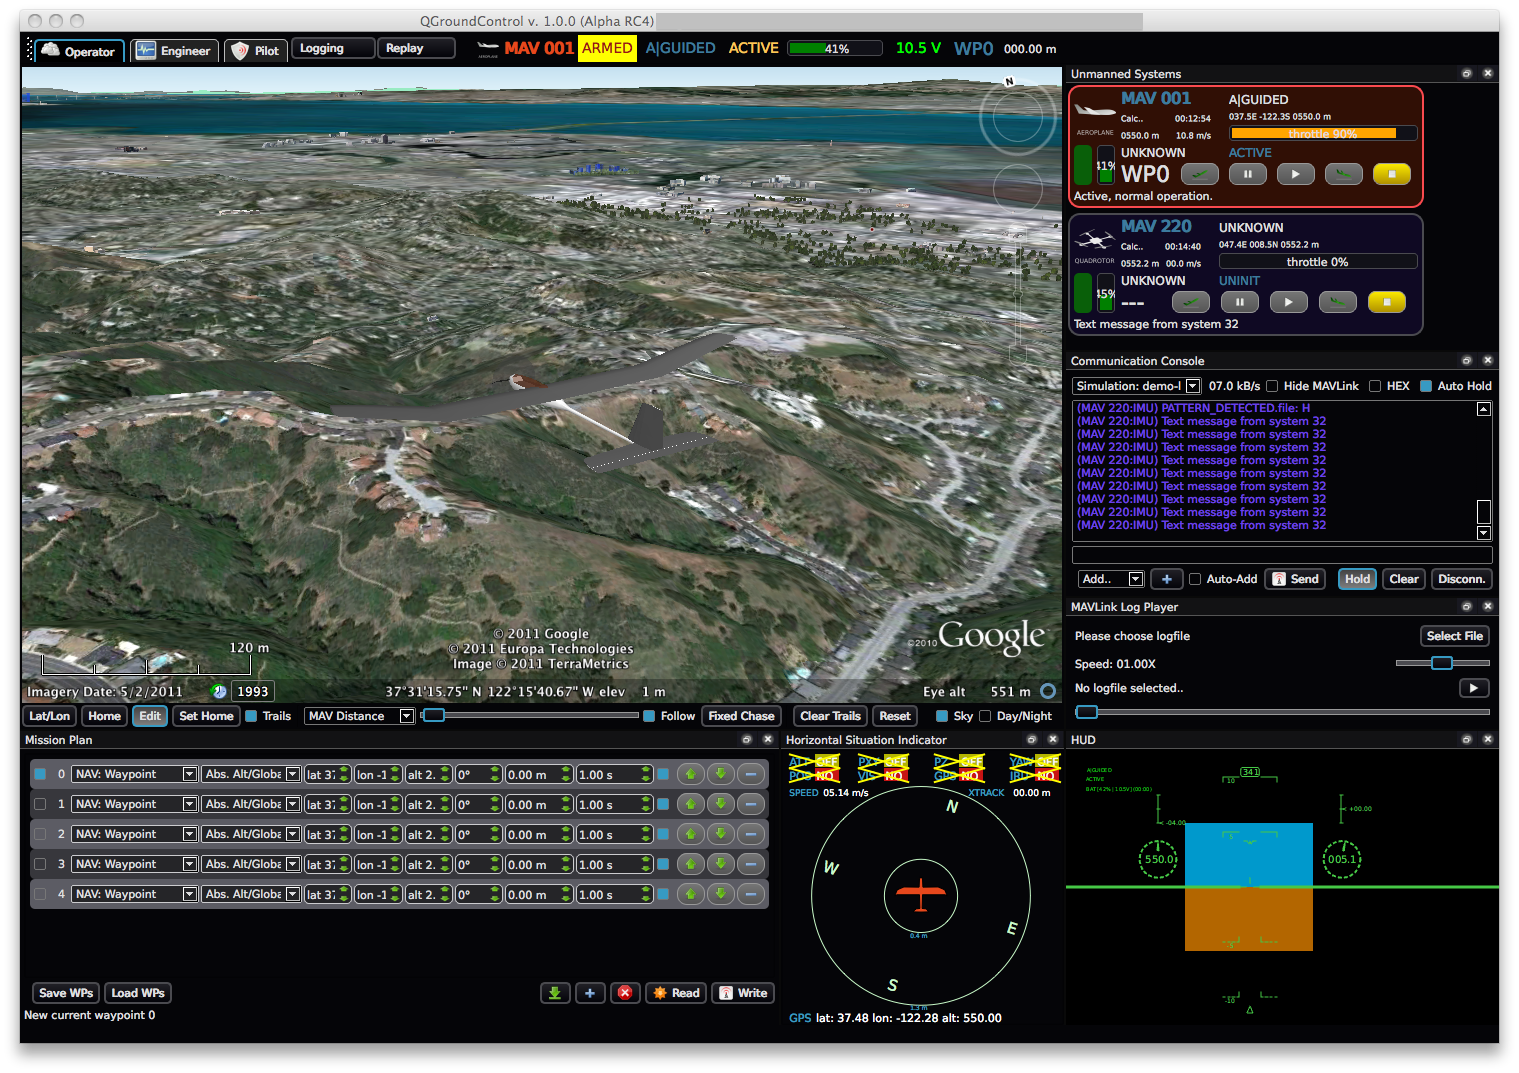
\includegraphics[width=1.0\textwidth]{QGC}
\end{figure}

The visual information from the incoming video in an interface can be presented in two different ways, \emph{egocentric} or \emph{exocentric}. Intuitively one is led to believe that an operator interface should mirror as closely as possible the view of a pilot on-board an aircraft, but contrary to that intuition Wang (2004) showed that egocentric views are not always the preferable option \cite{31}. The two approaches have their advantages and drawbacks leading to trade-off decisions related to the desired performance between the local and global awareness. One approach is to give the operator the ability to switch between the two views as needed, but in that case we need to take into consideration the extra workload that results from context-switching or mentally integrating the two views. 

The research has shown that the content and format of information displayed in the interface has a potentially large effect on the system's performance level \cite{1, 2}. The information that is well organized, provides enough concrete details, is consistent, etc, tends to increase the level of trust that the operator has for the system. Baker \emph{et al.} (2004) have shown the importance of integrating visual information from incoming video with the other robot sensor information \cite{22}. Their study revealed that during a disaster mitigation mission most of the users, except for those highly experienced, focused solely on the video-stream window, while neglecting the other information on the interface screen. In the other hand, simply incorporating all the necessary information around the video-window is not a solution becuase it may overload the display and thereof increase the workload on the human operator. To overcome the issue of increased monitoring requirements it is desirable to “hide” certain information from the user and utilize “alarm-systems” to notify the operators as needed about the critical events that need their attention. This leads to another research question related to what type of information can be "hidden", and at what mission stages can this information be "hidden" without having any negative impact on the system performance in general, as well as on the operator's situational awareness in specific? 

Another human factor to be considered is related to the question of what sensory input should be used to communicate important information to the operator, visual (pop-up windows), auditory, or a combination of both? Audio alerts introduce less overload on the operator, but in the other hand they provide less situational awareness as the operator needs to distinguish what a given signal is telling them. Wickens (2002) suggests that cross-modal approach (information divided between one visual and one auditory channel) is better than intra-modal (e.g. two visual channels) \cite{3}. Finding the trade-off between these two factors is an interesting topic that needs to be further investigated through experimentation. Further work needs to be done in order to determine precisely what type of information is best presented visually and what through audio signals, and how to integrate the two sensory inputs to achieve an improved situational awareness while reducing the operator workload. 

Endsley (2000) has suggested that goals are crucial in the development of SA. In a goal-driven process, the operators tend to search for the information related to the goal and to build goal-driven mental models that are used to filter and interpret the information \cite{26}. Many other researchers claim that humans built mental models that shape how they filter, understand, and interpret the information they receive. Therefore, when designing an interface it is important to have a sound understanding of how first responders model the process of a disaster mitigation response, and to design the interface accordingly so it fits these mental models. 

In a disaster scenario the emergency personnel on the ground will often have the need to task a robot to a specific location (e.g. to get additional information before the human responders decide to enter a potentially hazardous area). With a centralized control approach, whenever such a need becomes apparent the first responders have to contact the ground control station, explain their need for tasking a robot to the specific area, give coordinates of the area, and wait for the GCS operator to accomplish the requested action. This scenario introduces communication overload, delay in response times, and additional load on the GCS human operator, therefore, it is desirable to have the possibility for the emergency personnel to task the robots directly from the ground. Prior work has shown a positive response from first responders in regard to the portability of the interface \cite{25}. However, switching the UAV control between the operator at the ground station and emergency personnel on the ground may have significant negative impact on the situational awareness of the operator, which is another human factor implication that needs to be taken into account when designing the HRI interfaces for disaster mitigation. 

In conclusion, the open research questions related to the design of interfaces for UAV control include: 
\subsection{Interface Design Open Questions}
\begin{description}

	\item[$\bullet$] 
	What is the appropriate trade-off between egocentric and exocentric views in the operator interface? 
	\item[$\bullet$] 
	What are the possible approaches to integrating these views without introducing additional cognitive load on the human operator?
	\item[$\bullet$] 
	What is the appropriate interface content and format to ensure the appropriate level of operator trust? 
	\item[$\bullet$] 
	What is the best form of presenting information to the operator (visual vs audio)? In what situations is one approach better than the other?
	\item[$\bullet$] 
	What are the most appropriate audio alerts to ensure that that the operator has clear understanding of what these signals mean? 
	\item[$\bullet$] 
	How to capture the mental-models that the first responders have about a disaster mitigation operation? How to use these models to build an interface using a goal-driven approach? How will the goals affect the SA? 
	\item[$\bullet$] 
	What is the effect of the team on SA? i.e. how will an operator's situational awareness be affected by the fact that first responders on the ground have the ability to control the UAVs directly? 
	
\end{description}

\section{AUTONOMY}
The level of autonomy is another deterministic factor for the overall performance of the unmanned aerial systems. Autonomous navigation and control has been the focus of  many researchers during the past decade. Engel \emph{et al.} focused their work in developing a system able to navigate autonomously through previously unknown environment using a monocular camera as its main sensor \cite{13, 14, 15}. Autonomous navigation was also the subject addressed by the research conducted by Saska \emph{et al.} \cite{27}, as well as Achtelik \emph{et al.} who focused on tracking and control of UAVs using the readings from a stereo camera system and inertial sensors \cite{21}. In the initial phases of UAV development all unmanned aircrafts were \emph{teleoperated} (remotely controlled) by a human operator, but with the recent research achievements we are starting to see more and more UAVs that are capable of navigating and accomplishing tasks in a fully autonomous fashion. Nevertheless, as we discussed earlier neither teleoperation nor full autonomy are desired approaches for the control of UAVs in a disaster mitigation operation. It is well known that automated systems are governed by a formal syntax that limits their flexibility to address certain situations, hence it is necessary to always have a human operator ready to take over and handle the situation when automation reaches its limits. Automation has clear advantages in terms of, for instance, precision and overload, but in the other hand previous research has shown that the emergency personnel has no trust in fully autonomous systems, therefore they prefer teleoperated, semi-autonomous, rather than autonomous ones \cite{7}. Riley (1994) showed that trust is the main factor that determines if an operator will chose to use an optional automation or refuse to accept its usefulness altogether. Research has shown that both extremes of trust can be potentially dangerous for the success of the mission. Insufficient trust can lead to situations where the operator refuses to make use of automation \cite{30}, while in the other hand over-trust may lead the operator to rely on automation even in situations when better performance would be achieved if the human took control over the system \cite{4}. These issues need to be taken into account when designing the human-UAV interaction strategies, and this leads to an important research question: how to establish the appropriate balance between automation and human control in order to achieve maximum trust and acceptance for the UAS? \cite{17} 

Automation also influences the level of workload on human operators. While intuitively we might think that higher automation by default means less overload, this is not always the case. Automation can often have the effect of merely changing the nature of workload (reduce manual load while increasing the cognitive load), or shifting the workload in time (support the pilot at times of low workload but fail to do so when needed most). The research has shown that increased automation might in occasions have such negative effect, thus the UAV system should be designed not only to avoid overload, but under-load as well \cite{9}. 

\begin{figure}[h!]
  \caption{Autonomy vs Situational Awareness}
  \centering
    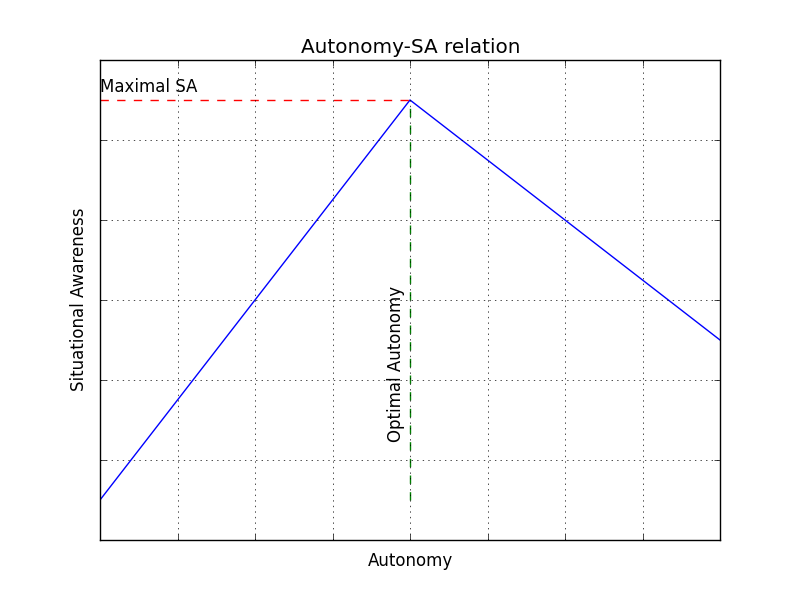
\includegraphics[width=0.75\textwidth]{autonomy}
\end{figure}

Another implication of the automation is related to the human alertness or situational awareness during the disaster mitigation mission. Namely, an early work by Bainbridge (1987) \cite{20} has proven the weakness of humans to maintain their attention during the periods of low task demand. This is another reason why the possible under-load should be taken into account because it may result with reduced situational awareness, hence failure of human operator to observe important (even critical) moments during an disaster mitigation mission. The effects of automation on autonomy are best described through the graph in Fig 2. From the figure we can see that the SA increases linearly with autonomy up until the point when in reaches the maximal SA. Increasing the autonomy beyond this point has the negative effect of reduced SA because of the low task demands. Further research should be conducted in order to \emph{optimal autonomy} level that ensures the maximal SA in a disaster mitigation scenario. 

\subsection{Automation Research Questions}

\begin{description}
	\item[$\bullet$] 
	What is the appropriate level of automation that ensures a balanced operator trust? 
	\item[$\bullet$] 
	What are the appropriate tasks to be automated, and to what level should they be automated in order to achieve a reduced operator workload?
	\item[$\bullet$] 
	What are the best ways to maintain the operators alertness throughout the different phases of UAV operation? 
	\item[$\bullet$]
	How to determine the optimal autonomy that ensures the maximal level of situational awareness? 
\end{description}

\section{PERFORMANCE METRICS}
An important area that also needs to be considered is related to the metrics used for validation of human-UAV interfaces. Measuring the operator's workload and situational awareness becomes difficult from the fact that both these measures are subjective in nature, and they depend largery on the operator training, experience, cognitive abilities, and so on. Murphy (2010) emphasized the importance of designing common metrics that would become the standard for evaluating HRI aspects in the robot-assisted SAR systems \cite{28}. However, until now no such a standard has been established and researchers use different metrics that are often contradictory, evaluate interfaces incorrectly, or evaluate one aspect of human-robot interaction correctly but fail to properly validate the system as a whole. 

The experiments related to human-UAV interaction generally tend to validate the interfaces in terms of \emph{implicit performance measures} and \emph{subjective measures}. The first method attempts to evaluate situational awareness through the measurement of the operational performance, implying that better SA leads to better performance \cite{12}. Several researchers have taken the approach of measuring the system performance, hence workload and situational awareness, in terms of time required for an operator to learn using the interface, time to complete a given mission, and minimization of \emph{critical incidents} during the operation \cite{18}. However though, we feel that using operational performance as a metric for SA and workload should be avoided because it might often lead to incorrect conclusions. Instead, we encourage the use of objective measures that tend to capture the SA and workload directly rather than as functions of operational performance. 

\subsection{Operator Workload}
Operator workload can be defines as the level of work/attention required from the operator in order to complete the mission in a successful and efficient way. When designing a UAV system the goal is to reduce the workload as less workload means an operator can control an incrased number of UAVs. However though, one should be careful not to reduce the workload at the levels that would have negative impact in the situational awareness as discussed in the previous sections. Finding the balance between the reduced workload and increased SA is an interesting research topic that needs to be investigated further. 

An interesting objective measure for the operator workload is proposed by Olsen \& Goodrich \cite{5}. They used the concepts of \emph{neglect tolerance} and \emph{interaction effort} as measures to evaluate the quality of human-robot interface in terms of operator workload. Neglect tolerance is defined as a measure of how the robot's current effectiveness declines as a function of time since the user last paid attention to the robot \cite{5}. 

The most commonly used subjective measure to capture the operator workload is the NASA-TLX, which assesses the operator's perceived workload in terms of mental demands, physical demands, temporal demands, own performance, effort, and frustration \cite{29}.

\subsection{Situational Awareness}  
When discussing the situational awareness of the human operator, the most commonly cited definition is the one given by Endsley \cite{34}: 

\emph{\begin{center}The perception of the elements in the environment within a volume of time and space, the comprehension of their meaning and the projection of their status in the near future.\end{center}}

\begin{figure}[h!]
  \caption{Situational Awareness, Endsley(1995)}
  \centering
    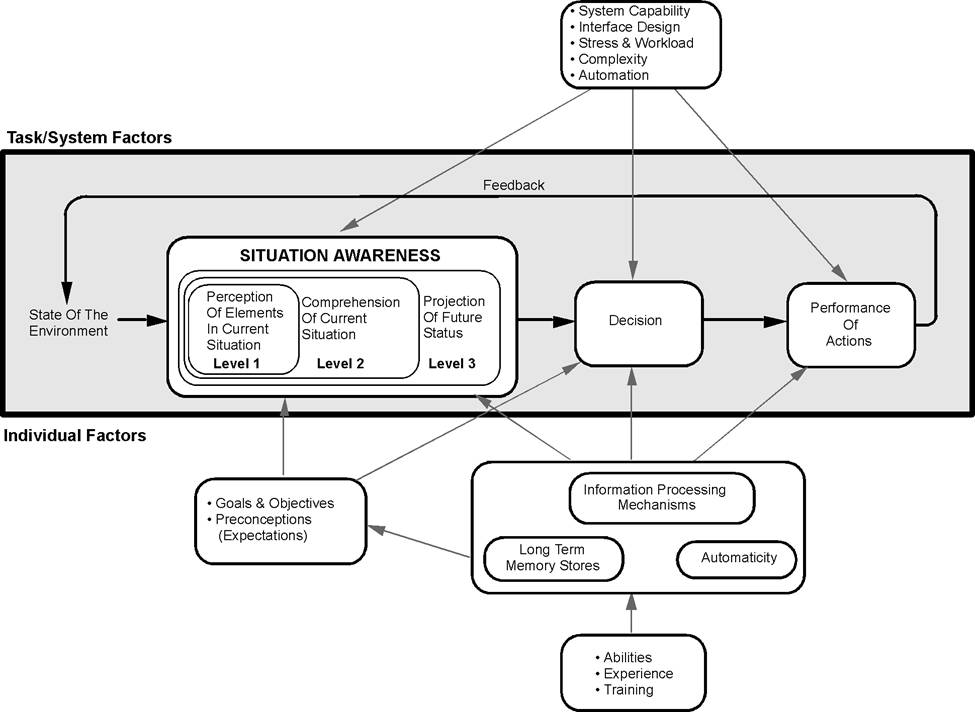
\includegraphics[width=0.75\textwidth]{SA_95}
\end{figure}

Based on the SA definition and Figure 3 we can say that meauring the situational awareness is equivalent to measuring the operators ability to perceive relevant information in
the environment, next to integrate the data in conjunction with task goals, and finally, at its
highest level, to predict future events and system states based on this understanding.

The most common objective measure for SA is based on Endsley's definition and is called \emph{Situation Awareness Global Assesment Technique} (SAGAT). In SAGAT, the simulation is paused and the display is blanked while questions regarding the situation are asked. Once a participant answers all the questions, the simulation is resumed only to be stopped again at some later point for additional SAGAT questions. The level of SA is measured as a number of correctly answered questions and the time taken to answer the questions \cite{34}. 

Another similar objective measure is the \emph{Situation Present Awareness Method (SPAM)} \cite{35}. The difference from SAGAT is that in SPAM the simulation is not paused and the questions are administered verbally (e.g. through headphones) whenever the participants indicate they are ready to answer. Two measures are collected during this test, the number of correct answers and the SPAM latency, or otherwise the amount of time it takes on average to respond correctly.   

Visser \emph{et al.} proposed the concepts of \emph{mission model memory} and \emph{deviation detection} as objective measurements for interface usability. The goal of this approach is to asses if the participants can remember which tasks were executed, which agent was responsible for each tasks, and how the tasks were related, which would in turn serve as an indicator of their situational awareness \cite{6}. 

In the other hand subjective measures are SA measurement techniques that aim to evaluate people's self-assessment of the SA \cite{12}. In the past the SA has been measured using techniques as direct interviews with the human operators \cite{7}. One technique for measuring the operator's self-perceived SA is the \emph{Situation Awareness Rating Technique (SART)}. The SART questionnaire requires participants to rate demand on attentional resources, supply of attentional resources and understanding of the situation on a 1-7 scale. Responses to the SART result in a subscale for each of the aforementioned dimensions as well as a combined score based on the difference between attentional demand and the sum of supply and understanding ratings \cite{36}. 

Another subjective measure of SA is the \emph{China Lake Situational Awareness (CLSA)}, a 10 point rating scale developed by the Naval Air Warfare Center. The CLSA is a questionaire administered upon completion of the mission and it captures the operators self-perceived situational awareness during the mission \cite{37}.

\subsection{Metrics Research Questions}

\begin{description}
	\item[$\bullet$]
	What are the best objective and subjective metrics to capture the operators' workload? 
	\item[$\bullet$]
	What are the best objective and subjective metrics to capture the operators SA? 
	\item[$\bullet$]
	What is the combination of metrics that best evaluate the human factors in UAV interfaces as an aggregate combination of effectiveness, workload, and situational awareness? 
	
\end{description}

\section{CONCLUSIONS}
Operator workload and situational awareness have been proven to be the key challenges to robot-assisted disaster mitigation \cite{18}. Both overload and SA depend on operator training, experience, noises, stress, distractions, etc, but they also depend largely on the design decisions related to human factors for UAS. In this review we have discussed the human factors (workload and SA) in terms of interface design and autonomy. We have tried to give a review of the current state in these areas and identify possible future research that would address important challenges with the purpose of improving the quality of human-UAV interaction in a disaster mitigation scenario. The potential research areas that we identified include several questions related to the content and format of the information presented in a human-UAV interface, as well as to the levels of autonomy that are most appropriate to ensure a reduced operator workload while maintaining high situational awareness. At the last section we also discussed several objective and subjective metrics that we feel are the most appropriate to correctly quantify the operator workload and SA during a disaster mitigation mission. Our future work will be focused on designing and conducting a number of experiments with a goal of answering the research questions identified here. Our experimental resutls will be reported in the subsequent papers and our work will culminate with the design and implementation of a UAV control interface that, based on our experimental results, ensures an intuitive control of multiple UAV in a disaster mitigation scenario.   

\medskip
\pagebreak

\bibliographystyle{plain}
\bibliography{review}

\end{document}